% context: 9th-grade physics homework, first problem set of Unit 2 (kinematics),
%        Giancoli 2-1 reference frames and displacement
% topic: drawing vectors on 2-D axes, reading vectors off a grid, adding displacements
%        back and forth along one line, distance vs displacement, a moving reference frame
% structure: two pages; page 1 vectors on a grid, page 2 one-dimensional motion.
%        No 2-D vector addition yet.
\documentclass[12pt, twoside]{article}
%\documentclass[12pt, twoside]{article}
\usepackage[letterpaper, margin=1in, headsep=0.2in]{geometry}
\setlength{\headheight}{0.6in}
%\usepackage[english]{babel}
\usepackage[utf8]{inputenc}
\usepackage{microtype}
\usepackage{amsmath}
\usepackage{amssymb}
%\usepackage{amsfonts}
\usepackage[nomessages]{fp} %\FPeval{\var-name}{2*sin(pi/6)}
\usepackage{siunitx} %units in math. eg 20\milli\meter
\usepackage{yhmath} % for arcs, overparenth command
\usepackage{tikz} %graphics
\usetikzlibrary{quotes, angles, arrows, arrows.meta}
\usepackage{graphicx} %consider setting \graphicspath{{images/}}
\usepackage{parskip} %no paragraph indent
\usepackage{enumitem}
\usepackage{multicol}
\usepackage{venndiagram}

\usepackage{fancyhdr}
\pagestyle{fancy}
\fancyhf{}
\renewcommand{\headrulewidth}{0pt} % disable the underline of the header
\raggedbottom
\hfuzz=2mm %suppresses overfull box warnings

\usepackage{hyperref}
\usepackage{float}

\title{Physics}
\author{Chris Huson}
\date{October 2026}

\fancyhead[LE]{\thepage}
\fancyhead[RO]{\thepage \\ Nickname: \hspace{2.25cm} \,\\ \,}
\fancyhead[LO]{La Scuola d'Italia / Huson / Physics \\* 15 October 2026}

\begin{document}

\subsubsection*{2.1 Homework: Reference Frames and Displacement}

\textbf{Reference (provided).} \quad
displacement $=$ final position $-$ starting position \\
distance $=$ total length of the path traveled

\vspace{0.2cm}

\begin{enumerate}[itemsep=0.5cm]

\item On the grid, each square is 1 m, $+x$ is east, and $+y$ is north. Starting
  from the origin, draw and label each displacement vector.

  \begin{minipage}[t]{0.42\linewidth}
    \vspace{0.2cm}
    $\vec{A}$: \; 4 m east \\[0.25cm]
    $\vec{B}$: \; 3 m north \\[0.25cm]
    $\vec{C}$: \; 5 m west \\[0.25cm]
    $\vec{D}$: \; 2 m south \\[0.25cm]
    $\vec{E}$: \; from the origin to $(-3,\, 4)$

    \vspace{0.6cm}

    \begin{enumerate}[itemsep=0.8cm]
      \item $\vec{E}$ is \rule{1cm}{0.4pt} m west, \\[0.3cm]
        and \rule{1cm}{0.4pt} m north.
      \item How long is $\vec{E}$?
    \end{enumerate}
  \end{minipage}
  \hfill
  \begin{minipage}[t]{0.54\linewidth}
    \vspace{0pt}
    \centering
    \begin{tikzpicture}[scale=0.55]
      \draw[gray!40, thin, step=1] (-6,-6) grid (6,6);
      \draw[->, thick] (-6.3,0) -- (6.6,0) node[right]{$x$};
      \draw[->, thick] (0,-6.3) -- (0,6.6) node[above]{$y$};
      \foreach \x in {-6,-4,-2,2,4,6} \node[below] at (\x,0) {\scriptsize \x};
      \foreach \y in {-6,-4,-2,2,4,6} \node[left] at (0,\y) {\scriptsize \y};
      % Solution vectors — uncomment to see the answer
      %\draw[->, very thick] (0,0) -- (4,0) node[near end, above]{$\vec{A}$};
      %\draw[->, very thick] (0,0) -- (0,3) node[near end, right]{$\vec{B}$};
      %\draw[->, very thick] (0,0) -- (-5,0) node[near end, above]{$\vec{C}$};
      %\draw[->, very thick] (0,0) -- (0,-2) node[near end, right]{$\vec{D}$};
      %\draw[->, very thick] (0,0) -- (-3,4) node[near end, left]{$\vec{E}$};
    \end{tikzpicture}
  \end{minipage}

\item Four vectors are drawn on the grid below. A vector is set by its length and its
  direction only --- it can be drawn anywhere.

  \begin{minipage}[t]{0.47\linewidth}
    \vspace{0pt}
    \centering
    \begin{tikzpicture}[scale=0.62]
      \draw[gray!40, thin, step=1] (0,0) grid (9,7);
      \draw[->, thick] (-0.3,0) -- (9.5,0) node[right]{$x$};
      \draw[->, thick] (0,-0.3) -- (0,7.5) node[above]{$y$};
      \foreach \x in {1,...,9} \node[below] at (\x,0) {\scriptsize \x};
      \foreach \y in {1,...,7} \node[left] at (0,\y) {\scriptsize \y};
      \draw[->, very thick] (1,1) -- (4,3) node[midway, above left]{$\vec{P}$};
      \draw[->, very thick] (5,1) -- (8,3) node[midway, below right]{$\vec{Q}$};
      \draw[->, very thick] (5,6) -- (2,4) node[midway, above left]{$\vec{R}$};
      \draw[->, very thick] (8,4) -- (8,7) node[midway, right]{$\vec{S}$};
    \end{tikzpicture}
  \end{minipage}
  \hfill
  \begin{minipage}[t]{0.49\linewidth}
    \vspace{0pt}
    \begin{enumerate}[itemsep=0.5cm]
      \item Describe each vector.

        \vspace{0.1cm}
        \renewcommand{\arraystretch}{1.6}
        \begin{tabular}{| c | c | c |}
          \hline
          & left/right & up/down \\ \hline
          $\vec{P}$ & & \\ \hline
          $\vec{Q}$ & & \\ \hline
          $\vec{R}$ & & \\ \hline
          $\vec{S}$ & & \\ \hline
        \end{tabular}
      \item Which two vectors are equal?
      \item Which vector is the opposite of $\vec{P}$?
    \end{enumerate}
  \end{minipage}

\newpage

\item Take the classroom door as the origin, with east positive. A student walks
  8 m east, then 5 m west, then 7 m west. Draw each displacement as an arrow above the
  number line, each one starting where the last one ended.

  \begin{center}
  \begin{tikzpicture}[scale=0.75]
    \draw[<->, thick] (-6.6,0) -- (10.6,0) node[right]{$x$ (m)};
    \foreach \x in {-6,...,10} \draw (\x,0.12) -- (\x,-0.12);
    \foreach \x in {-6,-4,...,10} \node[below] at (\x,-0.12) {\small \x};
    \node[above] at (0,0.1) {\scriptsize door};
    \path (0,0) -- (0,3.0); % room above the line for the arrows
    % Solution arrows — uncomment to see the answer
    %\draw[->, very thick] (0,0.8) -- (8,0.8) node[midway, above]{\small $+8$ m};
    %\draw[->, very thick] (8,1.6) -- (3,1.6) node[midway, above]{\small $-5$ m};
    %\draw[->, very thick] (3,2.4) -- (-4,2.4) node[midway, above]{\small $-7$ m};
  \end{tikzpicture}
  \end{center}

  \begin{enumerate}[itemsep=0.5cm]
    \item Where does the student end up? \hfill $x = $ \rule{2.5cm}{0.4pt}
    \item What is the student's displacement? \hfill \rule{3.5cm}{0.4pt}
    \item What distance did the student walk? \hfill \rule{3.5cm}{0.4pt}
  \end{enumerate}

\item Find the distance traveled and the displacement for each trip. Give a direction
  with each displacement that is not zero. A Manhattan block is about 80 m.

  \vspace{0.15cm}
  \renewcommand{\arraystretch}{1.75}
  \begin{tabular}{| l | p{0.115\linewidth} | p{0.19\linewidth} |}
    \hline
    \textbf{Trip} & \textbf{Distance} & \textbf{Displacement} \\ \hline
    (a) One lap of a 400 m running track & & \\ \hline
    (b) Empire State Building: 320 m up to floor 86 & & \\ \hline
    (c) Up to floor 86, then back down to the lobby & & \\ \hline
    (d) Manhattan: 10 blocks north, then 4 blocks south & & \\ \hline
  \end{tabular}

\item \textbf{Reference frames.} A Frecciarossa train travels north at 300 km/h
  relative to the ground.
  \begin{enumerate}[itemsep=0.55cm]
    \item A passenger sits in their seat. What is their speed relative to the train?
      Relative to the ground?
    \item The passenger walks at 5 km/h relative to the train. What is their velocity
      relative to the ground when they walk toward the front? Toward the back?
    \item A train going south at 300 km/h passes on the other track. How fast does
      it rush past, as seen by a seated passenger?
  \end{enumerate}

\end{enumerate}
\end{document}
